\documentclass[11pt]{article}

\usepackage{amsmath}
\usepackage{textcomp}
\usepackage[top=0.8in, bottom=0.8in, left=0.8in, right=0.8in]{geometry}
% add other packages here
\usepackage{indentfirst}
\usepackage{float}
\usepackage[usenames, dvipsnames]{color}

\usepackage{graphicx}
\graphicspath{ {./images/} }

\renewcommand{\labelitemi}{\textendash}

% put your group number and names in the author field
\title{\bf Exercise 2: A Reactive Agent for the Pickup and Delivery Problem}
\author{Group \textnumero:44 Valentin Kindschi, Cyril van Schreven}

% the report should not be longer than 3 pages

\begin{document}
\maketitle

\section{Problem Representation}

\subsection{Representation Description}
% describe how you design the state representation, the possible actions, the reward table and the probability transition table

We define $N$ as the total number of cities.\\

A \textit{state} $s$ is defined by the city the agent is at, and the task that it is offered. There is one distinct task per destination city, plus there is the possibility that there are no tasks available. There are thus $N+1$ states per city, and $N*(N+1)$ states in total.\\

An \textit{action} $a$ is a movement to another city. It is defined by a destination, and the carrying of a package or not.\\

The reward table $R(s,a)$ has a reward value for each combination of state and action. It accounts for the cost of travelling, and for the (optional) reward of a task.\\

Formally, the transition probability table $T(s,a,s')$ has a value for each combination of state, action, and next state. In our problem the transition is a movement to a new city. The transition is only non-deterministic because different tasks (or none) can be present at that city. The original state is not relevant. Also, the probability transition table has a distinct value for each destination city (action) and each possible state at that city, thus $N*(N+1)$ values.

\subsection{Implementation Details}
% describe the implementation details of the representations above and the implementation details of the reinforcement learning algorithm you implemented
First, note that even if there can be tasks of varying rewards going from origin city to another, this is not taken into account. These tasks are considered the same, and the average reward is used.\\

A state is implemented as a class \textit{ReactiveState} with three objects:
\begin{itemize}
    \item the current city, a \textit{City} object as defined in the logist.topology package.
    \item the presence of a task, a boolean.
    \item the destination city, a \textit{City} object as defined in the logist.topology package.
\end{itemize}
If there is no task available, the destination city is per definition null.\\

An action is implemented as a class \textit{ReactiveAction} with three objects:
\begin{itemize}
    \item the destination city, a \textit{City} object as defined in the logist.topology package.
    \item the use of a task, a boolean.
    \item the reward of the action, a double.
\end{itemize}
Note that a different \textit{ReactiveAction} instance is created for each state the action originates from. $N²*(N+1)$ instances are created. It is therefore possible for it to hold the reward value because it will depend on the departing and the destination cities.\\

Finally, some map objects are created to link the different states, actions and cities: \textit{statesInCity} links each city to its own list of states, \textit{possibleActions} links each city to its possible actions and \textit{strategy} links each state to the optimal action determined by the reinforcement learning algorithm.\\

The action reward is equal to $taskReward-cost$. The reward for a task is defined in the \textit{TaskDistribution} class in the logist.task package. The cost of a travel can be computed as the $costPerKm*distanceTravelled$. If an action is performed without task, the value of that action in the reward table will always be negative. Also, the reward table is not explicitly created. As mentioned above, the reward is saved within each instance of the action class.\\

The transition probability table is technically already implemented in the \textit{TaskDistribution} class in the logist.task package. Indeed, the action defines the transition to a new city. From that city, the task distribution to other cities defines the probability of each state to occur.

\section{Results}
% in this section, you describe several results from the experiments with your reactive agent

\subsection{Default setup}

The setup used for the experiments is the following:
\begin{itemize}
    \item The default settings: \textit{settings-default.xml}
    \item The topology of France: \textit{france.xml}
    \item A uniformly drawn probability distribution of task availability between 0 and 1.
    \item A constant reward distribution with a policy giving higher values to short distances, between 10000 and 99999.
    \item A uniformly drawn probability of there being no task between 0 and 1.
\end{itemize}


\subsection{Experiment 1: Discount factor}
% the purpose of this experiment is to understand how the discount factor influences the result

\subsubsection{Setting}
% you describe how you perform the experiment (you also need to specify the configuration used for the experiment)
All the parameters are fixed except the discount factor.

\subsubsection{Observations}
% you describe the experimental results and the conclusions you inferred from these results

As one can see on Figure (\ref{fig:dr}) below, there is almost no noticeable difference between the curves, excpet for the beginning, where the smallest discount factor takes more time to reach its steady state. This is surprising as the theory would predict that the agents with a higher discount factor look further in the potential future states and achieves better results on the long term. A possible explanation for this observation would be that the optimal strategy is rather greedy.

\begin{figure}[H]
	\centering
	%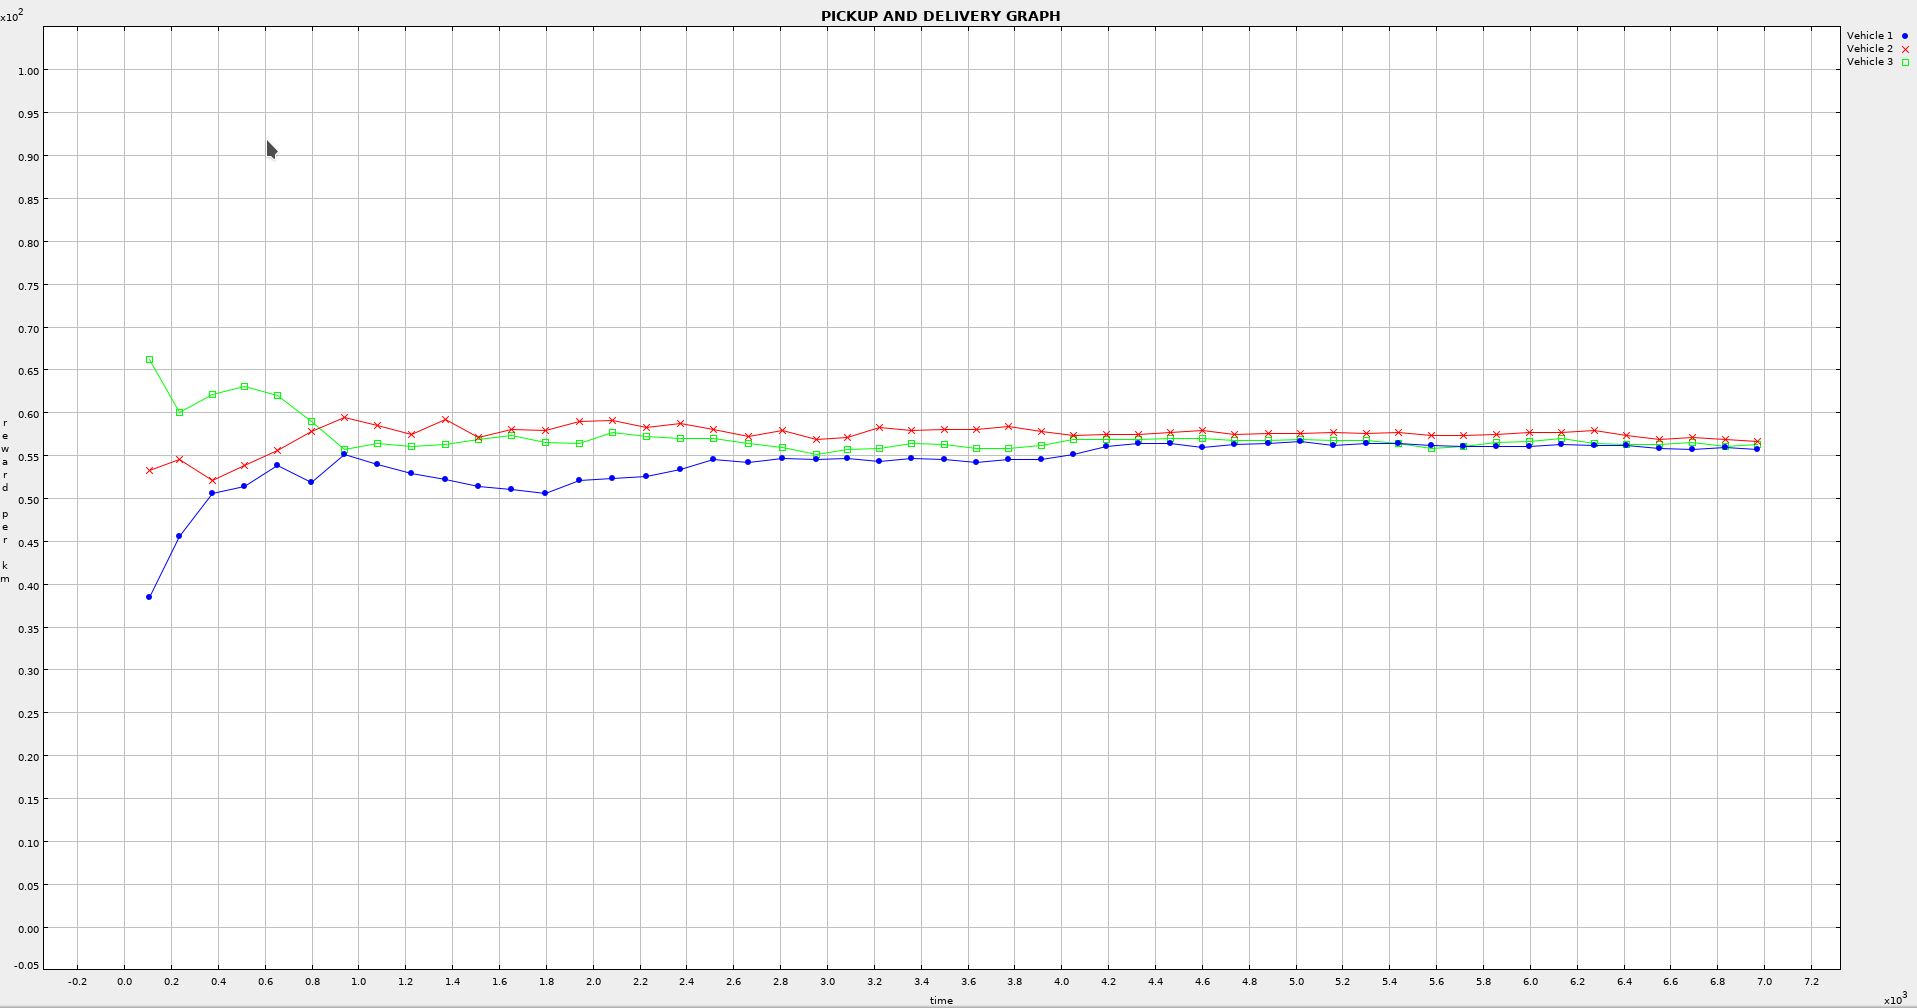
\includegraphics[scale = 0.25]{reduc_0-5_0-95_0-999.png}
	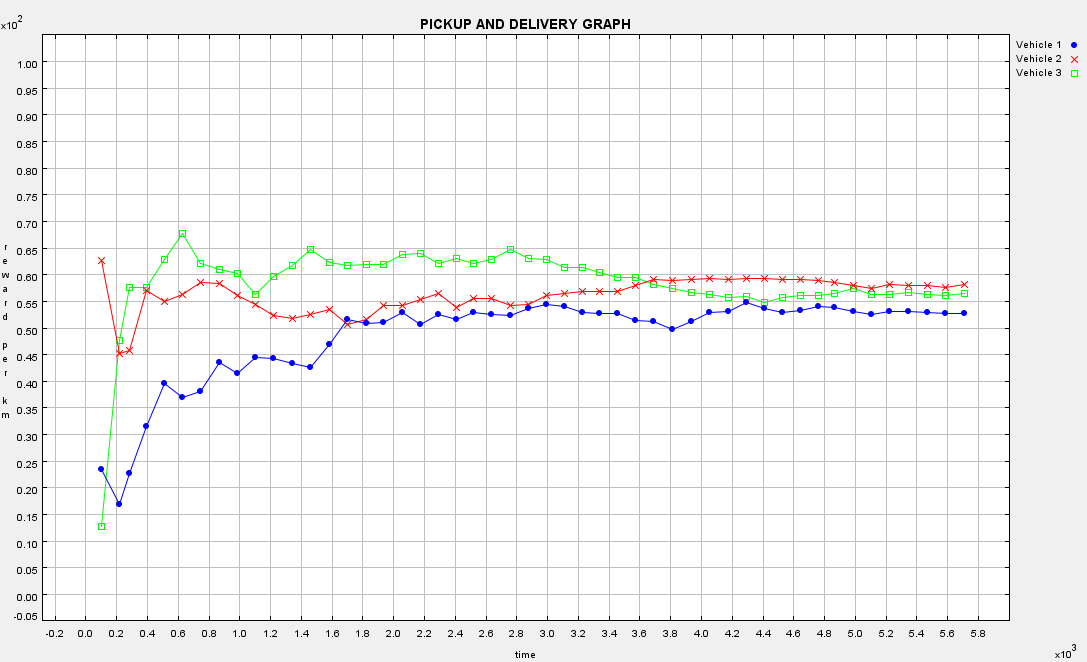
\includegraphics[scale = 0.44]{discount.PNG}
	\caption{Results with different discount rates (\textcolor{blue}{blue}: 0.5, \textcolor{red}{red}: 0.95, \textcolor{green}{green}: 0.999)}
    \label{fig:dr}
\end{figure}
    	
\subsection{Experiment 2: Comparisons with dummy agents}
% you compare the results of your agent with two dummy agents: the random agent that was already given in the starter files and another dummy agent that you define and create. You should report the results from the simulations using the topologies given in the starter files and optionally, additional topologies that you create.

\subsubsection{Setting}
% you describe how you perform the experiment and you describe the dummy agent you created (you also need to specify the configuration used for the experiment)
The reactive agent is compared with two dummy agents. The random agent and the neighbor agent. The neighbor agent accepts tasks if and only if they are to be deliver in a neighboring city.

\subsubsection{Observations}
% elaborate on the observed results

\begin{figure}[H]
	\centering
	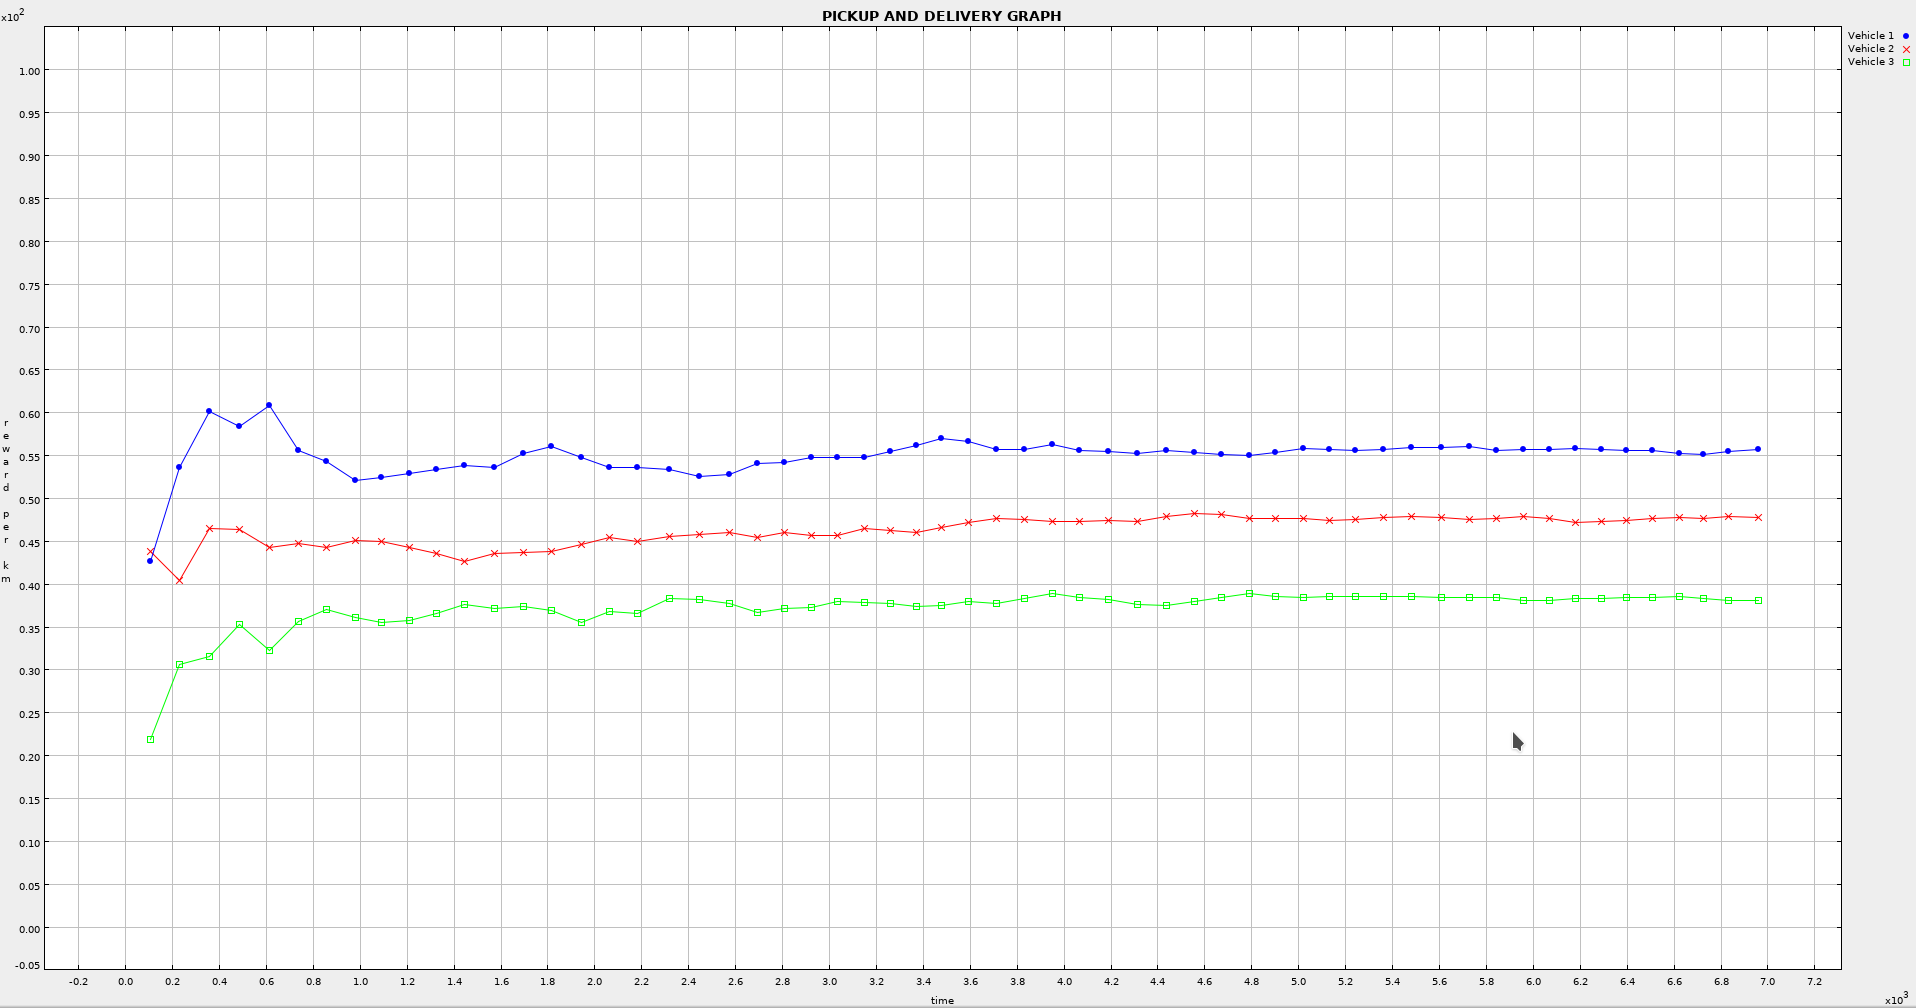
\includegraphics[scale = 0.25]{rla-random-neighbor.png}
\caption{Results with different agents (\textcolor{blue}{blue}: reactive (rla), \textcolor{red}{red}: random, \textcolor{green}{green}: neighbor)}
    \label{fig:exp2}
\end{figure}

The results shown on Figure (\ref{fig:exp2}) are clear. The reactive agent based on the reinforcement learning algorithm is the most cost efficient. The random agent comes second. A purely random agent would come lower but this agent takes the task 95/100 of the time. The neighbor agent comes last. This makes sense as it is an arbitrary rule and the agent refuses many potential rewards.

\end{document}